\section{Computational Complexity}
\paragraph{Problems:} informally, a problem is a \textbf{question} on a \textbf{system} of \textbf{mathematical objects}. The same question can often be asked on many similar systems
\begin{itemize}
	\item an \textbf{instance} $i \in I$ is each specific system concerned by the question 
	\item a \textbf{solution} $s \in S$ is an answer corresponding to one of the instances
\end{itemize}
Formally, a problem is the f\textbf{unction which relates instances and solutions}
$$ P : \, I \rightarrow S $$
Defining a function doesn't mean knowing how to compute it.\\

\paragraph{Algorithms:} an algorithm is a \textbf{formal procedure}, composed by \textbf{elementary steps}, in \textbf{finite sequence}, each determined by an input and by the results of the previous steps.\\

An algorithm for a \textbf{problem} $P$ is an algorithm which, given in \textbf{input} $i \in I$, returns in \textbf{output} $S_i \in S$
$$ A : \, \rightarrow S $$

An algorithm \textbf{defines a function} plus the \textbf{way to compute} it; it can be
\begin{itemize}
	\item \textbf{exact} if its associated function coincides with the problem
	\item \textbf{heuristic} otherwise
\end{itemize}
A heuristic algorithm is \textbf{useful} if it is
\begin{enumerate}
	\item \textbf{efficient:} it "costs" much less than an exact algorithm
	\item \textbf{effective:} it "frequently" provides a solution "close" to the right one
\end{enumerate}

\newpage

\subsection{Cost of an Algorithm}
The "cost" of an algorithm denotes the \textbf{computational cost} of running it: 
\begin{itemize}
	\item \textbf{space} occupied in memory
	\item \textbf{time} required to terminate
\end{itemize}
The \textbf{time} is usually considered more important, since: 
\begin{itemize}
	\item space is \textbf{renewable}, can be reused, time isn't 
	\item using \textbf{space} always \textbf{requires time}
	\item usage of space is usually \textbf{easier} to \textbf{distribute} (among machines)
\end{itemize}
Space and time are \textbf{partly interchangeable}, it's possible to reduce use of one by increasing the other.\\

Physical time is dependent on too many unreliable factors, and the measure of \textbf{computational time} should be 
\begin{itemize}
	\item \textbf{unrelated to technology}, i.e. the same for different machines
	\item \textbf{concise}, summarized in a simple symbolic expression
	\item \textbf{ordinal}, sufficient to compare different algorithms
\end{itemize}

\newpage

\subsection{Worst-case asymptotic time complexity}
The Worst-case asymptotic time complexity provides such a measure through the passages of:
\begin{enumerate}
	\item define the \textbf{time} $T$ as the \textbf{number of elementary operations} performed (independent from the specific machine)
	\item define the \textbf{size of an instance} as a suitable value $n$ (e.g. the number of elements in the ground set)
	\item find the \textbf{worst-case}, the maximum of $T$ \textbf{on all instances} of size $n$
	$$ T(n) = \max_{i \in I_n} T(i) \;\;\;\;\; n \in \mathbb{N} $$
	Now time complexity is a function $T : \, \mathbb{N} \rightarrow \mathbb{N}$.
	\item \textbf{approximate} $T(n)$ from above/below \textbf{with a simpler function} $f(n)$, considering only their \textbf{asymptotic behavior} (for $n \rightarrow +\infty$, we want an efficient algorithm on instances of large sizes)
	\item collect the function in \textbf{classes} with the \textbf{same approximating functions}
\end{enumerate}

\paragraph{$\Theta$ functional spaces:}
$$ T(n) \in \Theta(f(n))$$
Represents the \textbf{tight bound} of a function's growth rate, $T(n)$ must be "enclosed" between $c_1 f(n)$ and $c_2 f(n)$, from a "large" value of $n$, i.e. it's valid from a point $n_0$ forward.\\
Asymptotically, $f (n)$ \textbf{estimates} $T (n)$ up to a multiplying factor.

\paragraph{$O$ functional spaces:}
$$ T(n) \in O(f(n))$$
Represents the \textbf{upper bound} of a function's growth rate, $c \cdot f(n)$ "dominates" $T(n)$, from a point $n_0$ forward. \\
Asymptotically, $f (n)$ \textbf{overestimates} $T (n)$ up to a multiplying factor.

\paragraph{$\Omega$ functional spaces:}
$$ T(n) \in \Omega(f(n))$$
Represents the \textbf{lower bound} of a function's growth rate, $T(n)$ dominates $\Omega(n)$ from a point $n_0$ forward. \\
Asymptotically, $f (n)$ \textbf{underestimates} $T (n)$ up to a multiplying factor.

\newpage

\subsubsection{The exhaustive algorithm}
Within CO problems. Define the \textbf{size} of an instance as the \textbf{cardinality} of the \textbf{ground set}
$$ n = |B| $$
The exhaustive algorithm
\begin{itemize}
	\item considers \textbf{each} and every \textbf{subset} $x \subseteq B$, that is each $x \in 2^{|B|}$
	\item test its \textbf{feasibility} ($x \in X$) in time $\alpha (n)$
	\item if positive, \textbf{evaluates} the \textbf{objective} $f(x)$ in time $\beta(n)$
	\item \textbf{updates} the best value found so far, if needed
\end{itemize}
The \textbf{time complexity} becomes
$$ T(n) \in \Theta \left(2^n \left(\alpha (n) + \beta (n)\right)\right) $$
This is \textbf{at least exponential}, even if $\alpha (n)$ and $\beta(n)$ are small polynomials (which is often the case).\\

The exhaustive algorithm is impractical most of the time.

\subsubsection{Polynomial and exponential complexity}
In CO, the main \textbf{distinction} is between: 
\begin{itemize}
	\item \textbf{polynomial complexity:} $T(n) \in O (n^d)$ for a constant $d > 0$
	\item \textbf{exponential complexity:} $T(n) \in \Omega(d^n)$ for a constant $d > 1$
\end{itemize}
The \textbf{first} family includes \textbf{efficient} algorithms, the \textbf{second} \textbf{inefficient} ones.\\

In general, the \textbf{heuristic} algorithms are \textbf{polynomial} algorithms for problems whose known \textbf{exact} algorithms are all \textbf{exponential}.\\

\newpage

\subsection{Problem transformations and reductions}
Problems can be \textbf{transformed} into other problems (\hyperref[I5]{Interlude 5}). A \textbf{relation} among problems allows to design algorithms: 
\begin{itemize}
	\item by \textbf{transformation}: 
	\begin{enumerate}
		\item given $I_P$ (instance of $P$) \textbf{build} $I_Q$
		\item given $I_Q$, \textbf{apply} $A_Q$ to \textbf{obtain} $S_Q$ (solution of $I_Q$)
		\item given $S_Q$, \textbf{build} $S_P$
	\end{enumerate}
	\item by \textbf{reduction}: \textbf{repeat} the transformation, correcting $I_Q$ based on the \textbf{solutions obtained}; iterate the process
\end{itemize}

If $A_Q$ is exact/heuristic, $A_P$ is exact/heuristic.\\

The two algorithms often have a \textbf{similar complexity}, if $A_Q$ is polynomial/exponential and
\begin{itemize}
	\item building $I_Q$ takes polynomial time
	\item the number of iterations is polynomial
	\item building $S_P$ takes polynomial time
\end{itemize}
then $A_P$ is polynomial/exponential.\\

\newpage

\subsection{Beyond the worst-case complexity}
The worst-case complexity \textbf{cancels} all information on the \textbf{easier instances} (maybe i just need to use easy instances) and gives a rough \textbf{overestimate} of the computational time, in some (rare) case useless.\\

What if the \textbf{hard} instances are \textbf{rare} in practice? To \textbf{compensate} one can investigate: 
\begin{itemize}
	\item \textbf{parameterized complexity}, that is introduce some \textbf{other relevant parameter} $k$ (besides the size $n$) and express the \textbf{time as} $T(n,k)$
	\item \textbf{average-case complexity}, that is assume a \textbf{probability distribution} on $I$ and express the \textbf{time} as the \textbf{expected value}
	$$ T(n) = E \left[T(i) | i \in I_n \right] $$
\end{itemize}

\subsubsection{Parameterized complexity}
Some algorithms are \textbf{exponential} in $k$ an \textbf{polynomial} in $n$ and thus: 
\begin{itemize}
	\item \textbf{efficient} on instances with \textbf{low} $k$
	\item \textbf{inefficient} on instances with \textbf{large} $k$
\end{itemize}
\begin{center}
	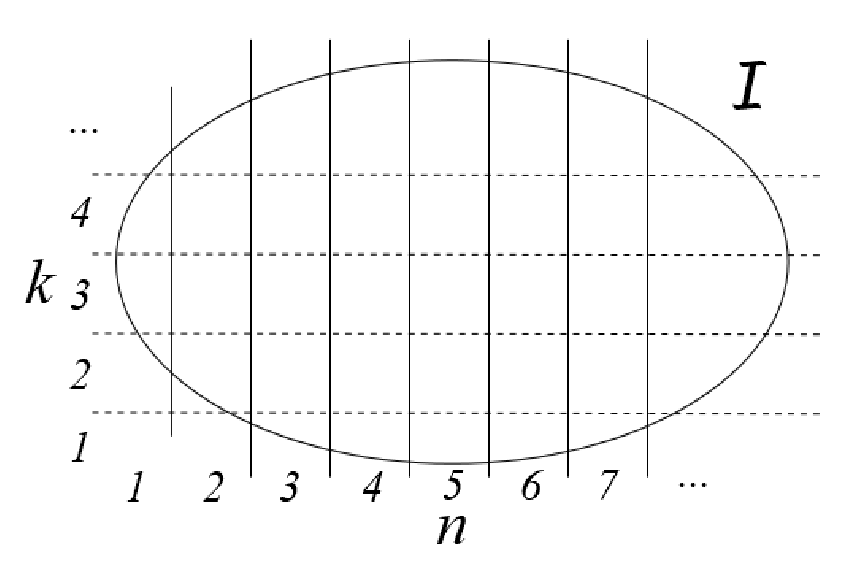
\includegraphics[width=0.5\columnwidth]{img/PC1}
\end{center}

\newpage

\paragraph{Nature of $k$:} it could be part of the \textbf{input}: 
\begin{itemize}
	\item a \textbf{numerical constant} (e.g. the capacity of the KP)
	\item the \textbf{maximum number of literals} per formula in logic function problems
	\item the \textbf{number on nonzero elements} in numerical matrix problems
	\item the \textbf{maximum degree}, \textbf{the diameter}, etc... in graph problems
\end{itemize}
one knows \textit{a priori} whether the algorithm is efficient on a given instance.\\

If the additional parameter $k$ is part of the \textbf{solution}: 
\begin{itemize}
	\item the \textbf{cardinality} of the solution
\end{itemize}
one will only find out \textit{a posteriori} (but an estimate \textit{a priori} could be available).\\

\paragraph{Example: the VCP;} \textbf{Exhaustive algorithm:} for each of the $2^n$ subsets of vertices, test if it covers all edges, compute its cardinality and keep the smallest one
$$ T(n,m) \in \Theta \left(2^n (m+n)\right) $$
If we already know that there's a solution with $f(x) = |x| = k+1$, we can look for a solution of $k$ vertices, decreasing $k$ progressively; if we can't find it we already have the optimal solution.\\

\textbf{Naive algorithm:} for each subset of $k$ vertices, test if it covers all edges
$$ T(n,m,k) \in \Theta \left(n^k m\right) $$
for a fixed $k$, this algorithm is polynomial (but in general very slow).\\

\newpage

\textbf{Bounded tree search:} a better algorithm can be based on the following useful property
$$ x \cap (u,v) \neq \emptyset \text{ for all } x \in X, \, (u,v) \in E $$
Any feasible solution \textbf{includes} at least one \textbf{extreme vertex} for each edge.\\
Choose any edge (there can be "good" and "bad" edges), only one must be in the solution.\\

BTS algorithm to find $x$ with $|x| \leq k$:
\begin{enumerate}
	\item choose \textbf{any} $(u,v)$: either $u \in x$ or $u \notin x$ and $v \in x$ (there must be only one in the solution)
	\item for each open case, \textbf{remove} the \textbf{vertices} of $x$ and the \textbf{edges they cover}
	$$ V := V \setminus x \;\;\;\;\; E := E \setminus \left\{e \in E: \, e \cap x \neq \emptyset \right\}$$
	The edges covered by vertices in $x$ are no longer constraining
	\item if $|x| \leq k$ and $E = \emptyset$, $x$ is the \textbf{required solution}; if the partial solution has $k$ elements (or less) and there are no more edges to cover then it's not a partial solution, it's a feasible one
	\item if $|x| \leq k$ and $E \neq \emptyset$, there is \textbf{no solution}
	\item otherwise go to step 1
\end{enumerate}
The \textbf{complexity} is $T(n,m,k) \in \Theta(2^k m)$, polynomial in $n$ ($m < n^2$). \\
For $n>>2$, this algorithm is much more efficient than the naive one.\\

\newpage

\subsubsection{Kernelization (or "problem reduction")}
Kernelization \textbf{transforms} all \textbf{instances} of $P$ into \textbf{simpler} instances of $P$ (also known as "problem reduction"), instead of instances of another problem $Q$.\\

Quite often, in fact, useful \textbf{properties} allow to \textbf{prove that}
\begin{itemize}
	\item there exists an optimal solution (not every optimal solution, but at least one) \textbf{not including} certain elements of $B \implies$ such elements can be \textbf{removed}
	\item there exists an optimal solution \textbf{including} certain elements of $B \implies$ such elements can be set \textbf{apart and added later}
\end{itemize}
In short, remove elements of $B$ without affecting the solution.\\

Possible useful \textbf{outcomes} are
\begin{itemize}
	\item an \textbf{exact} algorithm \textbf{polynomial} in $n$ (the problem becomes simpler, parameterized complexity)
	\item \textbf{faster} exact and heuristic algorithms (the instance is smaller so it's faster and usually better since the smaller problem is less "confusing")
	\item \textbf{better} heuristic \textbf{solutions}
	\item \textbf{heuristic kernelization:} apply \textbf{relaxed conditions} sacrificing optimality (risk losing the optimal solution but simplify the problem)
\end{itemize}

\newpage

\paragraph{Kernelization of VCP:} if $\delta_v \geq k+1$ (the degree of $v$, number of vertices), vertex $v$ belongs to any feasible solution of value $\leq k$ (you need to cover a lot of edges, this covers a lot of edges; by contradiction, you can't cover $k+1$ edges with less than this single vertex).\\

Kernelization algorithm to \textbf{keep} only \textbf{vertices of solution} $x$ with $|x| \leq k$
\begin{itemize}
	\item start at \textbf{step} $t = 0$ with $k_0 = k$ and an \textbf{empty} vertex \textbf{subset} $x_t := \emptyset$
	\item \textbf{set} $t = t + 1$ and \textbf{add} to the solution the \textbf{vertices of degree} $\geq k_t + 1$
	$$ \delta_v \geq k+1 \implies x_t := x_{t-1} \cup \left\{v\right\} $$
	\item \textbf{update} $k_t := k_0 − |x_t|$
	\item \textbf{remove} the \textbf{vertices} of \textbf{zero degree}, those \textbf{of} $x$ and the \textbf{covered edges}
	$$ V := \left\{v \in V : \, \delta_v > 0\right\} \setminus x_t \;\;\;\;\; E := \left\{e \in E : \, e \cap x_t = \emptyset \right\} $$
	\item if $|E| > k_t^2$ there is \textbf{no feasible solution} ($k_t$ vertices are not enough)
	\item if $|E| \leq k_t^2 \implies |V| \leq 2k_t^2$; \textbf{apply} the \textbf{exhaustive} algorithm
\end{itemize}
The \textbf{complexity} is $T(n,k) \in \Theta \left(n + m + 2^{2k^2}k^2 \right)$ (the last part is the one of the exhaustive algorithm, good if $k$ is small).\\

\textbf{Essentially:} it chooses the nodes with the most edges connected to them, removes them (and the nodes left with no edges), decreases the number of edges "required" to be "chosen" and starts again.\\

\newpage

\subsubsection{Average-case complexity}
Some algorithms are inefficient only on a few instances (see simplex algorithm for Linear Programming).\\

\textbf{Idea:} define time as the \textbf{expected value} of $T(i)$ on $I_n$ for each $n \in \mathbb{N}$
$$ T(n) = E \left[T(i) | i \in I_n \right]$$
\textbf{Theoretical} studies can define a \textbf{probabilistic model} of the problem, that is a probability \textbf{distribution} on $I_n$ for each $n \in \mathbb{N}$ (probability of each instance, typically quite simple, could be equiprobability) and \textbf{compute} the \textbf{expected value} of $T(I)$.\\

\textbf{Empirical} studies
\begin{itemize}
	\item build a \textbf{simulation model} of the problem, that is a probability distribution on $I_n$ for each $n \in \mathbb{N}$, let it be theoretical or empirical (drawn from real-world data) 
	\item build a \textbf{benchmark} of \textbf{random} instances according to the \textbf{distribution}
	\item apply the algorithm and \textbf{measure} the \textbf{time} required
\end{itemize}

\paragraph{Probabilistic models for numerical matrices:} Binary random matrix with a given size ($m$ rows and $n$ columns), some models are: 
\begin{enumerate}
	\item \textbf{equiprobability:} list all $2^{mn}$ binary matrices and select one of the matrices with uniform probability
	\item \textbf{uniform probability:} set each cell to $1$ with a given probability $p$
	$$ Pr[a_{ij} = 1] = p \;\;\;\;\; (i = 1, \, ... \, , m; \, j = 1, \, ... \, , n) $$
	If $p = 0.5$, it coincides with the equiprobability model, for other values some instances are more likely than others
	\item \textbf{fixed density:} extract $\delta mn$ (obviously $0 < \delta < 1$) cells out of $mn$ with uniform probability and set them to $1$.\\
	If $\delta = p$, it resembles the uniform probability model, but some instances cannot be generated
\end{enumerate}

\newpage

\paragraph{Probabilistic models for graph:} Random graph with a given number of vertices $n$, some models are: 
\begin{enumerate}
	\item \textbf{equiprobability:} list all $2^{\frac{n(n-1)}{2}}$ graphs and select one of the graphs with uniform probability
	\item \textbf{Gilbert’s model}, or \textbf{uniform probability} $G (n, p)$:
	$$ Pr  \left[(i,j) \in E \right] = p \;\;\;\;\; \left(i \in V , \, j \in V \setminus \left\{i\right\}\right)$$
	All graphs with the same number of edges $m$ have the same probability $p^m (1 − p)^{\frac{n(n-1)}{2} - m}$ (different for each $m$).\\
	If $p = 0.5$, it coincides with the equiprobability model
	\item \textbf{Erd\H{o}s-R\'enyi model} $G (n, m)$: extract $m$ unordered vertex pairs out of $\frac{n(n-1)}{2}$ with uniform probability and create an edge for each one
	If $\frac{2m}{n(n-1)} = p$, it resembles the uniform probability model, but some instances cannot be generated
\end{enumerate}

\paragraph{Probabilistic models for logic functions:} Random CNF with a given number of variables $n$ and a given number of literals $k$ for each logic formula
\begin{enumerate}
	\item \textbf{fixed-probability ensemble:} list all $\left(\begin{array}{c} n \\ k\end{array}\right) 2^k$ formulae of $k$ distinct and consistent literals and add each one to the CNF with probability $p$
	\item \textbf{fixed-size ensemble:} build $m$ formulae, adding to each one $k$ distinct and consistent literals, extracted with uniform probability.\\
	If $p = \frac{m}{\left(\begin{array}{c} n \\ k\end{array}\right) 2^k}$, it resembles the fixed-probability model, but some instances cannot be generated
\end{enumerate}

\newpage

\subsubsection{Phase transitions}
Different values of the (deterministic or probabilistic) \textbf{parameters} correspond to \textbf{different regions} of the \textbf{instance} set.\\
If you introduce parameters, different regions of the instance set are obtained.\\

For \textbf{graphs}
\begin{itemize}
	\item $m = 0$ and $p = 0$ correspond to \textbf{empty graphs}
	\item $m = \frac{n(n−1)}{2}$ and $p = 1$ correspond to \textbf{complete graphs }
	\item intermediate values correspond to graphs of \textbf{intermediate density} (deterministically for $m$, probabilistically for $p$)
\end{itemize}
You can expect the algorithm to perform differently on different regions.\\

For many problems the \textbf{performance} of algorithms is strongly \textbf{different in different regions} concerning
\begin{itemize}
	\item the \textbf{computational time} (for exact and heuristic algorithms)
	\item the \textbf{quality of the solution} (for heuristic algorithms)
\end{itemize}
Often, the performance \textbf{variation} takes place \textbf{abruptly} in \textbf{small regions} of the parameter space, as in phase transitions of physical systems (e.g. ice to water happens in a restricted zone).\\
This is useful to predict the behavior of an algorithm on a given instance.\\

\newpage

\paragraph{Phase transitions for 3-SAT and Max-3-SAT:} Given a CNF on $n$ variables, with logic formulae containing $3$ literals
\begin{itemize}
	\item \textbf{3-SAT:} is there a truth assignment satisfying all formulae?
	\item \textbf{Max-3-SAT:} what is the maximum number of satisfiable formulae?
\end{itemize}
As the formulae/variables ratio, $\alpha = m/n$, increases
\begin{itemize}
	\item \textbf{satisfiable instances decrease} from nearly all (many variables for few formulae) to nearly none (few variables for many formulae)
	\item the \textbf{computing time} first \textbf{sharply increases}, then \textbf{decreases} for SAT, increases further for Max-SAT (using a well-known exact algorithm)
\end{itemize}
\begin{center}
	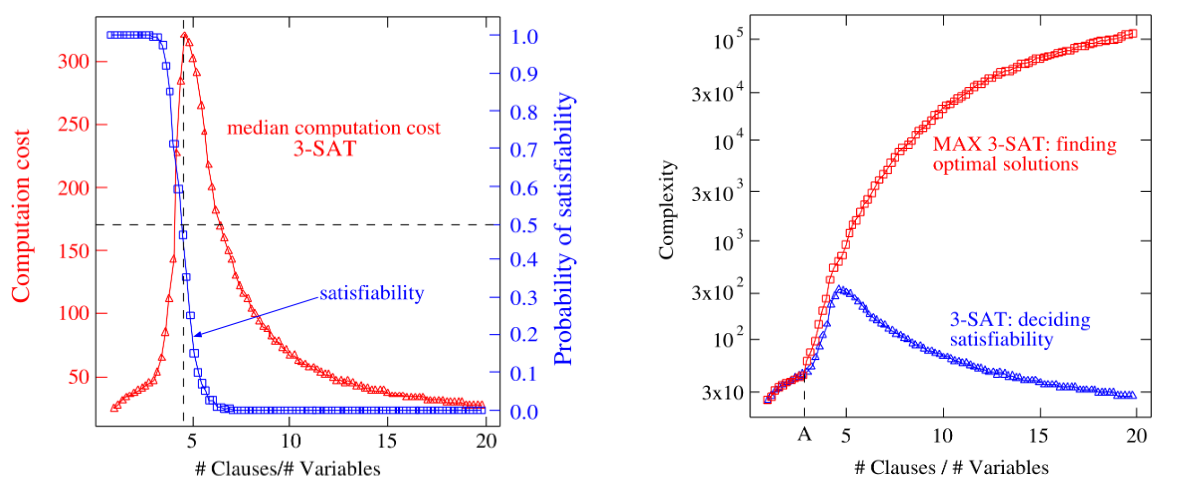
\includegraphics[width=\columnwidth]{img/PhaseT1}
\end{center}
The blue profile in the first graph (3-SAT) shows the number of instances that can be satisfied for a certain number of clauses/variables. The red shows the computational time (on a specific algorithm, but many have the same basic ideas), which starts small, gets big and then decreases (as stated before), there's a range, where the lines meet, which makes it hard to prove the satisfiability of the clauses.\\

In second graph (Max-3-SAT) the blue profile shows the complexity of deciding satisfiability (same as red in the first graph, re-scaled), the red one shows the complexity of finding optimal solutions, which only increases.\\

As $n \rightarrow + \infty$, the transition \textbf{concentrates} around $\alpha_c \approx 4.26$.\\

\newpage

\paragraph{Phase transition for the VCP:} The \textbf{VCP} exhibits a \textbf{similar phase transition} as $|x|/|V|$ increases, the computational time first explodes, then drops, as $n \rightarrow +\infty$ \textbf{concentrates} around a critical value.
\begin{center}
	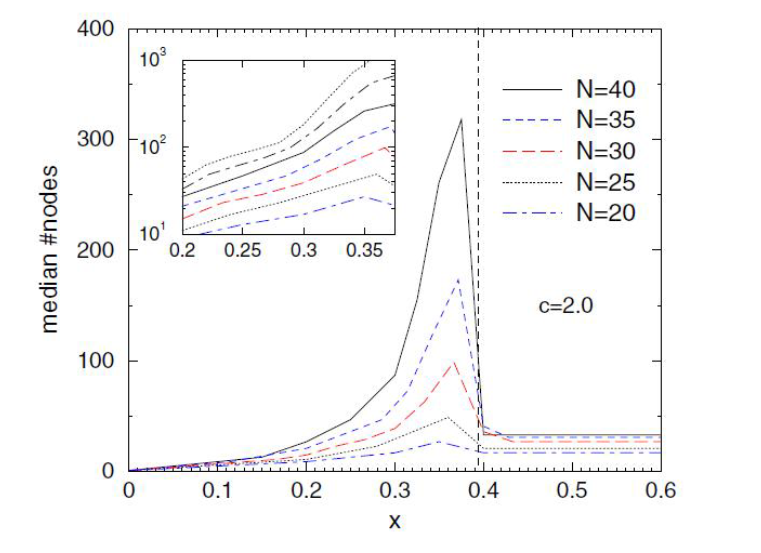
\includegraphics[width=0.7\columnwidth]{img/PhaseT2}
\end{center}
When $|x|/|V|$ is small some vertices are clearly necessary, when it's large many vertices are clearly necessary; in both cases, problem solved.\\

\vfill 

\subsection*{Computational cost of heuristic algorithms}
\addcontentsline{toc}{subsection}{Computational cost of heuristic algorithms}
The \textbf{time complexity} of a heuristic algorithm is usually
\begin{itemize}
	\item \textbf{strictly polynomial} (with low exponents)
	\item fairly \textbf{robust} with respect \textbf{to secondary parameters}
\end{itemize}
Therefore, the worst-case estimation is also good on average.\\

\textbf{Metaheuristics} use random steps or memory
\begin{itemize}
	\item the \textbf{complexity} is \textbf{well defined} for \textbf{single components} of the algorithm
	\item the \textbf{overall complexity} is \textbf{not clearly defined}
	\begin{itemize}
		\item in \textbf{theory}, it could extend \textbf{indefinitely} (but the pseudo-random number generator or the memory configurations would yield an infinite loop)
		\item in \textbf{practice}, it is defined by a \textbf{condition} imposed by the \textbf{user} 
	\end{itemize}
\end{itemize}

% End of L3

\newpage